\section{Deferred results and proofs}\label{app:proofs}

This appendix contains proofs and refinements for factorization non-identifiability, stable source-center capacity, cross-space accessibility, retained resolution, and estimation.

\section{Factorization non-identifiability}\label{app:discrepancy}


\subsection{Proof of Theorem~\ref{thm:discrepancy}}
\begin{proof}
Let $(h,p)$ and $(\widetilde h,\widetilde p)$ be admissible pairs satisfying
\[
\widetilde p(\widetilde h(V))=p(h(V))
\]
pathwise. They therefore induce exactly the same projected random variables. Since $J$ depends on the backbone and projector only through those projected variables,
\[
J(\widetilde h,\widetilde p)=J(h,p).
\]
If a backbone property takes different values on two admissible factorizations of the same projected map, the same objective value is compatible with both values. Hence that property cannot be uniformly certified by the $Z$-only objective.

The three examples in the main text are instances of this factorization ambiguity. An admissible bijection $\varphi$ gives the compensated reparameterization
\[
\widetilde h=\varphi\circ h,
\qquad
\widetilde p=p\circ\varphi^{-1}.
\]
More generally, if a possibly non-injective map $\varphi$ satisfies $p=q\circ\varphi$ on $\range(h)$, then
\[
\widetilde h=\varphi\circ h,
\qquad
\widetilde p=q
\]
leaves the projected variables unchanged while potentially discarding backbone information. Conversely, if
\[
\widetilde h(V)=(h(V),u(V)),
\qquad
\widetilde p(x,y)=p(x),
\]
then arbitrary additional information can be appended to the retained representation without changing $Z$ or the objective.
\end{proof}


\begin{corollary}[Projected Gaussianity does not transfer]\label{cor:gaussian}
Let $Z=(Z_1,Z_2)^\top\sim\mathcal N(0,I_2)$ and define
\[
H=
\begin{pmatrix}
Z_1\\
Z_2+Z_1^2-1
\end{pmatrix},
\qquad
p(h_1,h_2)=
\begin{pmatrix}
h_1\\
h_2-h_1^2+1
\end{pmatrix}.
\]
Then $p(H)=Z$ pathwise, but $H$ is non-Gaussian and
\[
\Cov(H)=\diag(1,3).
\]
Thus even exact isotropic Gaussianity in $Z$ certifies neither Gaussianity nor isotropy in $H$.
\end{corollary}

\begin{proof}
Direct substitution gives $p(H)=Z$. The second coordinate of $H$ contains the non-Gaussian random variable $Z_1^2-1$, so $H$ is not jointly Gaussian. Moreover,
\[
\Var(Z_2+Z_1^2-1)
=
\Var(Z_2)+\Var(Z_1^2)
=1+2=3,
\]
and
\[
\Cov(Z_1,Z_2+Z_1^2-1)=0.
\]
Thus $\Cov(H)=\diag(1,3)$.
\end{proof}


\begin{corollary}[Projected linear separability does not transfer]\label{cor:separability}
Let $X,R$ be independent Rademacher variables, let the label be $Y=X$, and define
\[
Z=(X,R)^\top,
\qquad
H=(XR,R)^\top,
\qquad
p(h_1,h_2)=(h_1h_2,h_2)^\top.
\]
Then $p(H)=Z$ pathwise. The label is linearly separable in $Z$ by the first coordinate, whereas the four support points of $H$ form an XOR configuration and are not linearly separable.
\end{corollary}

\begin{proof}
Because $R^2=1$,
\[
p(H)=(XR^2,R)=(X,R)=Z.
\]
The first coordinate of $Z$ equals $Y$, so $Z$ is linearly separable. In $H$, the positive-class points are $(1,1)$ and $(-1,-1)$, while the negative-class points are $(-1,1)$ and $(1,-1)$. If an affine score $a h_1+b h_2+c$ strictly separated the classes, the two positive inequalities would imply $2c>0$, whereas the two negative inequalities would imply $2c<0$, a contradiction.
\end{proof}


\section{Stable source-center capacity}\label{app:capacity}

We record the paired-view and finite-view statements for $B_s=\Cov(m_s(Q))$ and total within-source covariance $A_s$, the full moment-control consequence, and secondary conditioning corollaries. Appendix~\ref{app:resolution} develops the retained-backbone split of $A_s$ into structured view difficulty and excess thickness.


\begin{proposition}[Paired views separate stable spread from cloud thickness]\label{prop:paired}
Let $S_1,S_2$ be conditionally independent views given $Q$. Then
\[
B_s=\E[(S_1-\mu_s)(S_2-\mu_s)^\top],
\qquad
A_s=\frac12\E[(S_1-S_2)(S_1-S_2)^\top].
\]
\end{proposition}

\begin{proof}
Write $S_i=m_s(Q)+\xi_i$, with $\E[\xi_i\mid Q]=0$. Conditional independence gives $\E[\xi_1\xi_2^\top\mid Q]=0$, so all terms involving residuals vanish in the cross-covariance and
\[
\E[(S_1-\mu_s)(S_2-\mu_s)^\top]=B_s.
\]
Also $S_1-S_2=\xi_1-\xi_2$. The two conditional residual covariances add while their cross terms vanish, hence
\[
\frac12\E[(S_1-S_2)(S_1-S_2)^\top]=A_s.
\]
\end{proof}


\begin{proposition}[Pooled-center covariance equals stable spread plus $(1/V)$ thickness]\label{prop:finite-centers}
Let $S^{(1)},\ldots,S^{(V)}$ be conditionally independent views given the same source $Q$, and define the pooled center
\[
\overline S_V=\frac1V\sum_{v=1}^V S^{(v)}.
\]
Then
\[
\E[\overline S_V]=\mu_s,
\qquad
\widetilde B_{s,V}:=\Cov(\overline S_V)
=B_s+\frac1V A_s.
\]
Thus a covariance loss across $V$-view pooled centers targets $\widetilde B_{s,V}$, with residual averaging noise $A_s/V$.
\end{proposition}

\begin{proof}
Write $\overline S_V=m_s(Q)+\overline\xi_V$, where $\overline\xi_V=V^{-1}\sum_v\xi^{(v)}$ and $\E[\overline\xi_V\mid Q]=0$. By the law of total covariance,
\[
\Cov(\overline S_V)=B_s+\E[\Cov(\overline\xi_V\mid Q)].
\]
Conditional independence makes the covariance of the average equal to the average covariance divided by $V$, so
\[
\E[\Cov(\overline\xi_V\mid Q)]
=
\frac1V\E[\Cov(S\mid Q)]
=
\frac1V A_s.
\]
Thus $\Cov(\overline S_V)=B_s+A_s/V$.
\end{proof}


\begin{theorem}[Finite-view center moment control protects population center rank]\label{thm:kl}
Let
\[
\widetilde B_V=B+\frac1V A,
\qquad A\succeq0,
\]
on a $d$-dimensional active subspace. If
\[
\cK_{\rm ctr}(\mu,\widetilde B_V)\le\varepsilon,
\]
then $\norm{\mu}^2\le2\varepsilon$ and every eigenvalue of $\widetilde B_V$ lies in $[\ell_\varepsilon,u_\varepsilon]$, where $\ell_\varepsilon\le1\le u_\varepsilon$ solve
\[
x-\log x-1=2\varepsilon.
\]
If additionally $\norm{A}_{\mathrm{op}}\le\alpha<V\ell_\varepsilon$, then
\[
\left(\ell_\varepsilon-\frac{\alpha}{V}\right)I_d
\preceq B\preceq u_\varepsilon I_d,
\]
so $B$ is full rank and
\[
\srank(B)
=
\frac{\tr B}{\norm{B}_{\mathrm{op}}}
\ge
 d\,\frac{\ell_\varepsilon-\alpha/V}{u_\varepsilon}.
\]
\end{theorem}

\begin{proof}
Let $\widetilde\lambda_1,\ldots,\widetilde\lambda_d$ be the eigenvalues of $\widetilde B_V$. Then
\[
2\cK_{\rm ctr}(\mu,\widetilde B_V)
=
\norm{\mu}^2+
\sum_{j=1}^d
\bigl(\widetilde\lambda_j-\log\widetilde\lambda_j-1\bigr).
\]
The scalar function $f(x)=x-\log x-1$ is nonnegative, tends to infinity as $x\downarrow0$ or $x\uparrow\infty$, and vanishes only at $x=1$. Since every term is nonnegative, $\cK_{\rm ctr}(\mu,\widetilde B_V)\le\varepsilon$ implies $\norm{\mu}^2\le2\varepsilon$ and
\[
f(\widetilde\lambda_j)\le2\varepsilon
\]
for every $j$, hence
\[
\ell_\varepsilon I_d
\preceq
\widetilde B_V
\preceq u_\varepsilon I_d.
\]
Because
\[
B=\widetilde B_V-\frac1V A
\]
and $0\preceq A\preceq\alpha I_d$,
\[
B
\succeq
\ell_\varepsilon I_d-\frac{\alpha}{V}I_d
=
\left(\ell_\varepsilon-\frac{\alpha}{V}\right)I_d,
\qquad
B\preceq\widetilde B_V\preceq u_\varepsilon I_d.
\]
Therefore
\[
\tr B
\ge
 d\left(\ell_\varepsilon-\frac{\alpha}{V}\right),
\qquad
\norm{B}_{\mathrm{op}}
\le u_\varepsilon,
\]
which gives the stable-rank bound.
\end{proof}


\begin{proof}[Proof of Proposition~\ref{prop:capacity-main}]
Equation~\eqref{eq:pooled-cov-main} gives
\[
I_d=B_s+\frac1V A_s.
\]
Therefore
\[
B_s=I_d-\frac1V A_s.
\]
Since $0\preceq A_s\preceq\alpha I_d$,
\[
\left(1-\frac{\alpha}{V}\right)I_d
\preceq B_s\preceq I_d.
\]
The stable-rank bound follows from
$\tr B_s\ge d(1-\alpha/V)$ and $\norm{B_s}_{\rm op}\le1$.
\end{proof}


\begin{corollary}[Moment control bounds linear-probe sensitivity]\label{cor:probe-robustness}
Assume Theorem~\ref{thm:kl} holds for the backbone center covariance $B_h$ on a $d_h$-dimensional active subspace, and write
\[
\kappa_h=\ell_\varepsilon-\frac{\alpha_h}{V_h}>0.
\]
For a scalar source-level score $Y=Y(Q)$ with finite variance, let $(w_\star,b_\star)$ be the population least-squares affine predictor from the retained representation $H$. Since $C_h=B_h+A_h$,
\[
\norm{w_\star}^2
\le
\frac{(u_\varepsilon+\alpha_h)\,\Var(Y)}{\kappa_h^2}.
\]
For any additive perturbation $\eta$ to the retained representation, with second-moment matrix $M_\eta=\E[\eta\eta^\top]$,
\[
\E\!\left[\left(w_\star^\top(H+\eta)+b_\star-\bigl(w_\star^\top H+b_\star\bigr)\right)^2\right]
\le
\norm{M_\eta}_{\mathrm{op}}
\frac{(u_\varepsilon+\alpha_h)\,\Var(Y)}{\kappa_h^2}.
\]
If $\eta$ is additionally zero-mean and independent of $(H,Y)$, the same quantity is the increase in mean-squared prediction error of the fixed probe.
\end{corollary}

\begin{proof}
Since $C_h=B_h+A_h$, Theorem~\ref{thm:kl} and $0\preceq A_h\preceq\alpha_h I$ give
\[
\kappa_h I\preceq C_h\preceq (u_\varepsilon+\alpha_h)I.
\]
With an intercept, population least squares gives $w_\star=C_h^{-1}\Cov(H,Y)$ on the active subspace. Hence
\[
\norm{w_\star}
\le
\norm{C_h^{-1}}_{\mathrm{op}}\,\norm{\Cov(H,Y)}
\le
\frac{\sqrt{\norm{C_h}_{\mathrm{op}}\Var(Y)}}{\kappa_h}
\le
\frac{\sqrt{(u_\varepsilon+\alpha_h)\Var(Y)}}{\kappa_h},
\]
where the middle inequality is Cauchy--Schwarz. The perturbation bound follows from
\[
\E[(w_\star^\top\eta)^2]
=w_\star^\top M_\eta w_\star
\le\norm{M_\eta}_{\mathrm{op}}\norm{w_\star}^2.
\]
Under the stated independence and zero-mean condition, the cross term with the unperturbed regression residual vanishes.
\end{proof}


\section{Projected anchor and cross-space accessibility}\label{app:accessibility}

Using the established augmentation-operator viewpoint in spectral SSL \citep{haochen2021,balestriero2022,johnson2023,zhai2024}, define
\[
T:L^2_0(\nu)\to L^2_0(\pi),
\qquad
(Tf)(q)=\E[f(V)\mid Q=q],
\qquad
L_{\mathsf A}=I-TT^*.
\]
For each center-whitened projected coordinate, write
\[
\overline f_j(V):=\overline Z_j,
\qquad
\overline g_j(Q):=\E[\overline f_j(V)\mid Q]=\overline m_{z,j}(Q).
\]
Thus $\overline g_j=T\overline f_j$ and the $\overline g_j$ span $\cM_z$. The next bound translates normalized thickness $\Theta_z$ into this operator language.

\begin{proposition}[Projected thickness controls augmentation energy and tail localization]\label{prop:energy}
For the center-whitened projected center space $\cM_z$,
\[
\tr(P_{\cM_z}L_{\mathsf A})
=
\sum_{j=1}^{r_z}\ip{\overline g_j}{L_{\mathsf A}\overline g_j}
\le \tr\Theta_z.
\]
Consequently, if $P_{>\tau}$ denotes the spectral projector of $L_{\mathsf A}$ onto eigenvalues in $(\tau,1]$, then for every $\tau\in(0,1]$,
\[
\norm{P_{>\tau}P_{\cM_z}}_{\mathrm F}^2
\le
\frac{\tr\Theta_z}{\tau}.
\]
Thus small projected normalized thickness places most of $\cM_z$ in the low-frequency part of the augmentation operator.
\end{proposition}

\begin{proof}
Let $M=T^*T$. Since conditional expectation is a contraction, $0\preceq M\preceq I$. For any centered view function $f$ and $g=Tf$,
\[
\ip{g}{(I-TT^*)g}
=
\ip{f}{M(I-M)f}
\le
\ip{f}{(I-M)f}
=
\E[\Var(f(V)\mid Q)].
\]
Applying this to the coordinates $\overline f_j$ and summing gives the energy bound. The spectral theorem gives $L_{\mathsf A}\succeq\tau P_{>\tau}$, hence
\[
\tr(P_{\cM_z}L_{\mathsf A})
\ge
\tau\norm{P_{>\tau}P_{\cM_z}}_{\mathrm F}^2,
\]
which yields the tail bound.
\end{proof}


A standard eigengap comparison for equal-rank spectral subspaces gives the following localization statement.

\begin{theorem}[Projected spectral approximation for the two-space bridge]\label{thm:resolution}
Let $E_z\subset L^2_0(\pi)$ be an $r_z$-dimensional spectral subspace of $L_{\mathsf A}$ such that, for some $0\le a_z<b_z\le1$,
\[
P_{E_z}L_{\mathsf A}P_{E_z}\preceq a_zP_{E_z},
\qquad
P_{E_z^\perp}L_{\mathsf A}P_{E_z^\perp}\succeq b_zP_{E_z^\perp}.
\]
Set $\Delta_z=b_z-a_z>0$, $P_z=P_{\cM_z}$, and
\[
\varepsilon_{\rm proj}
:=
\tr\Theta_z-\tr(P_{E_z}L_{\mathsf A}).
\]
Then $\varepsilon_{\rm proj}\ge0$ and
\[
\norm{(I-P_{E_z})P_z}_{\mathrm F}^2
\le
\frac{\varepsilon_{\rm proj}}{\Delta_z}.
\]
Consequently, for every $y\in L^2_0(\pi)$ with $\norm{y}\le1$,
\[
\dist(y,\cM_z)
\le
\sqrt{\frac{\cE_{\mathsf A}(y)}{b_z}}
+
\sqrt{\frac{\varepsilon_{\rm proj}}{\Delta_z}}.
\]

\end{theorem}

\begin{proof}
Let $E=P_{E_z}$, $Q=I-E$, and $P=P_z$. Since $E_z$ is a spectral subspace, $E$ reduces $L_{\mathsf A}$. Because $E$ and $P$ have the same finite rank,
\[
D_z^2:=\tr(PQ)=\tr(E(I-P))=\norm{(I-E)P}_{\mathrm F}^2.
\]
The spectral separation gives
\[
\tr(PL_{\mathsf A})-\tr(EL_{\mathsf A})\ge\Delta_zD_z^2.
\]
Proposition~\ref{prop:energy} gives $\tr(PL_{\mathsf A})\le\tr\Theta_z$, so $D_z^2\le\varepsilon_{\rm proj}/\Delta_z$ and $\varepsilon_{\rm proj}\ge0$. Also,
\[
\norm{Qy}^2\le \frac{\cE_{\mathsf A}(y)}{b_z}.
\]
Using $PEy\in\cM_z$ and $\norm{(I-P)E}_{\rm op}=\norm{(I-E)P}_{\rm op}\le D_z$,
\[
\dist(y,\cM_z)
\le
\norm{Qy}+\norm{(I-P)Ey}
\le
\sqrt{\frac{\cE_{\mathsf A}(y)}{b_z}}+D_z,
\]
and substitution yields the claim.
\end{proof}


\subsection{Accessibility certificates}

\begin{proof}[Proof of Theorem~\ref{thm:accessibility}]
Population least squares makes $e_c$ uncorrelated with every coordinate of $m_h(Q)-\mu_h$. Therefore
\[
\Cov(\overline m_z)
=
\Cov\!\left(W_c(m_h-\mu_h)\right)+\Cov(e_c)
=
W_cB_hW_c^\top+\Sigma_c.
\]
Since the projected centers are whitened, $\Cov(\overline m_z)=I_{r_z}$, proving \eqref{eq:access-cov-decomp}.

Taking traces gives
\[
r_z=\tr(W_cB_hW_c^\top)+\tr\Sigma_c,
\]
which is part (i).

For part (ii), fix $u\in\R^{r_z}$. Multiplying the multivariate regression by $u^\top$ gives the scalar candidate coefficient $a=W_c^\top u$ and residual $u^\top e_c$. Least-squares orthogonality makes this scalar coefficient optimal, hence
\[
\min_a\E\!\left[
\bigl(u^\top\overline m_z-a^\top(m_h-\mu_h)\bigr)^2
\right]
=
\E[(u^\top e_c)^2]
=
u^\top\Sigma_cu.
\]

For part (iii), let $y_z=P_{\cM_z}y=u_y^\top\overline m_z$. The function $u_y^\top W_c(m_h-\mu_h)$ belongs to $\cM_h$, so the triangle inequality gives
\[
\begin{aligned}
 d_h(y)
&\le
\norm{y-y_z}_{L^2}
+
\norm{u_y^\top e_c}_{L^2}\\
&=
 d_z(y)+\sqrt{u_y^\top\Sigma_cu_y}.
\end{aligned}
\]
\end{proof}

\begin{corollary}[What high average accessibility implies]\label{cor:average-access-directions}
If $R^2_{\rm acc}\ge1-\delta$, then for every $\tau\in(0,1)$ at most $r_z\delta/\tau$ eigen-directions of $\Sigma_c$ have unexplained variance larger than $\tau$. Consequently,
\[
\rank(B_h)
\ge
r_z-\left\lfloor\frac{r_z\delta}{\tau}\right\rfloor.
\]
This controls most residual eigen-directions rather than the worst direction.
\end{corollary}

\begin{proof}
Let $\lambda_1,\ldots,\lambda_{r_z}$ be the eigenvalues of $\Sigma_c$. Since $R^2_{\rm acc}\ge1-\delta$ means $\sum_i\lambda_i=\tr\Sigma_c\le r_z\delta$,
\[
\#\{i:\lambda_i>\tau\}\,\tau
\le
\sum_{i:\lambda_i>\tau}\lambda_i
\le
r_z\delta.
\]
For every remaining eigenvector $q_i$, \eqref{eq:access-cov-decomp} gives
\[
q_i^\top W_cB_hW_c^\top q_i=1-\lambda_i\ge1-\tau>0.
\]
Thus $W_cB_hW_c^\top$, and hence $B_h$, has rank at least the number of such directions.
\end{proof}

\paragraph{Uniform center accessibility.}
For a worst-direction accessibility statement, assume the stronger certificate
\begin{equation}\label{eq:center-access-strong}
\norm{\Sigma_c}_{\rm op}\le\varepsilon_c^2,
\qquad \varepsilon_c<1.
\end{equation}

\begin{proposition}[Uniform center accessibility gives rank transfer and subspace containment]\label{prop:uniform-access}
Under \eqref{eq:center-access-strong},
\[
W_cB_hW_c^\top
\succeq
(1-\varepsilon_c^2)I_{r_z},
\qquad
\rank(B_h)\ge r_z,
\]
and
\[
\sup_{\substack{g\in\cM_z\\ \norm{g}=1}}
\dist(g,\cM_h)
\le\varepsilon_c.
\]
Consequently, for every centered $y$ with $\norm{y}\le1$,
\[
 d_h(y)\le d_z(y)+\varepsilon_c.
\]
Exact uniform accessibility implies $\cM_z\subseteq\cM_h$.
\end{proposition}

\begin{proof}
The covariance decomposition gives
\[
W_cB_hW_c^\top=I_{r_z}-\Sigma_c
\succeq
(1-\varepsilon_c^2)I_{r_z},
\]
which proves rank transfer. Every normalized $g\in\cM_z$ has the form $g=u^\top\overline m_z$ with $\norm{u}=1$. The candidate $\widetilde g=u^\top W_c(m_h-\mu_h)$ lies in $\cM_h$ and satisfies
\[
\norm{g-\widetilde g}_{L^2}^2
=u^\top\Sigma_cu
\le\varepsilon_c^2.
\]
The task bound follows from the same projection argument as Theorem~\ref{thm:accessibility}(iii). If $\varepsilon_c=0$, every $g\in\cM_z$ lies in $\cM_h$.
\end{proof}

The first subspace bound is the sine of the largest principal angle from $\cM_z$ to $\cM_h$ \citep{stewart2016cs}. Under exact accessibility, $\cM_z\subseteq\cM_h$ and the finite-dimensional center-function space admits the ordinary split
\[
\cM_h=\cM_z\oplus(\cM_h\cap\cM_z^\perp).
\]
For approximate accessibility, this is a principal-angle statement rather than an orthogonal decomposition of representation coordinates.

\paragraph{Viewwise accessibility.}
For the stronger individual-view relation, let
\[
W_v
=
\arg\min_W
\E\norm{\overline Z-W(H-\mu_h)}^2,
\qquad
r_v=\overline Z-W_v(H-\mu_h),
\]
and assume
\begin{equation}\label{eq:view-access}
\norm{\Cov(r_v)}_{\rm op}\le\varepsilon_v^2,
\qquad \varepsilon_v<1.
\end{equation}

\begin{proposition}[Viewwise accessibility transfers center geometry and accessible thickness]\label{prop:viewwise}
Under \eqref{eq:view-access},
\[
W_vB_hW_v^\top
\succeq
(1-\varepsilon_v)^2I_{r_z},
\]
and
\[
\norm{W_vA_hW_v^\top}_{\mathrm{op}}
\le
\left(\sqrt{\norm{\Theta_z}_{\mathrm{op}}}+\varepsilon_v\right)^2.
\]
In particular, the same map $W_v$ predicts the projected centers with residual covariance at most $\varepsilon_v^2I_{r_z}$.
\end{proposition}

\begin{proof}
Write
\[
e_v(Q)=\E[r_v\mid Q],
\qquad
\delta_v=r_v-e_v(Q).
\]
The law of total covariance gives
\[
\Cov(r_v)=\Cov(e_v)+\E[\delta_v\delta_v^\top].
\]
Hence both terms on the right are positive semidefinite and have operator norm at most $\varepsilon_v^2$.

Taking conditional expectations in
\[
\overline Z=W_v(H-\mu_h)+r_v
\]
gives
\[
\overline m_z(Q)=W_v(m_h(Q)-\mu_h)+e_v(Q).
\]
For any $u\in\R^{r_z}$, Minkowski's inequality yields
\[
\sqrt{u^\top W_vB_hW_v^\top u}
\ge
\sqrt{u^\top\Cov(\overline m_z)u}
-
\sqrt{u^\top\Cov(e_v)u}
\ge
(1-\varepsilon_v)\norm{u}.
\]
Since $\Cov(\overline m_z)=I_{r_z}$, squaring proves the center-rank bound.

Subtracting conditional means gives
\[
\overline Z-\overline m_z(Q)
=
W_v(H-m_h(Q))+\delta_v.
\]
For any unit vector $u$,
\[
\sqrt{u^\top W_vA_hW_v^\top u}
\le
\sqrt{u^\top\Theta_zu}
+
\sqrt{u^\top\E[\delta_v\delta_v^\top]u}
\le
\sqrt{\norm{\Theta_z}_{\rm op}}+\varepsilon_v.
\]
Taking the supremum over unit $u$ and squaring proves the thickness bound. The center residual statement follows from $\Cov(e_v)\preceq\Cov(r_v)$.
\end{proof}

\subsection{Deferred downstream consequences}
The following statements combine projected spectral approximation with center or viewwise accessibility from $H$.


\begin{proposition}[Probe error separates center approximation and cloud thickness]\label{prop:probe}
For a task score $Y=Y(Q)$ and an affine probe $w^\top H+b$,
\[
\E[(Y-w^\top H-b)^2]
=
\E[(Y-w^\top m_h(Q)-b)^2]+w^\top A_hw.
\]
If $|Y|\ge\gamma>0$, then
\[
\Pp\bigl(\sign(w^\top H+b)\ne\sign Y\bigr)
\le
\frac{\E[(Y-w^\top m_h(Q)-b)^2]+w^\top A_hw}{\gamma^2}.
\]
\end{proposition}

\begin{proof}
Write $H=m_h(Q)+\xi_h$. Expanding the squared loss, the cross term vanishes because $\E[\xi_h\mid Q]=0$, and the residual term is $w^\top A_hw$. A sign error implies
\[
|Y-(w^\top H+b)|\ge\gamma.
\]
Markov's inequality applied to the squared error proves the classification bound.
\end{proof}


\begin{theorem}[Uniform center accessibility yields a backbone regression bound]\label{thm:center-regression}
Assume Theorem~\ref{thm:resolution} and uniform center accessibility~\eqref{eq:center-access-strong}. Define
\[
\tau_{h\to z}^{(c)}:=\norm{W_cA_hW_c^\top}_{\rm op}.
\]
Let $Y=c+y(Q)$ with $y\in L^2_0(\pi)$ and $\norm{y}\le1$. Then there is an affine probe on $H$ satisfying
\[
\E[(Y-w^\top H-b)^2]
\le
\left(
\sqrt{\cE_{\mathsf A}(y)/b_z}
+
\sqrt{\varepsilon_{\rm proj}/\Delta_z}
+
\varepsilon_c
\right)^2
+
\tau_{h\to z}^{(c)}.
\]
\end{theorem}

\begin{proof}
Let
\[
y_z=P_{\cM_z}y=u^\top\overline m_z(Q).
\]
Because $\Cov(\overline m_z)=I_{r_z}$ and $\norm{y}\le1$,
\[
\norm{u}=\norm{y_z}\le1.
\]
Theorem~\ref{thm:resolution} gives
\[
\norm{y-y_z}
=
\dist(y,\cM_z)
\le
\sqrt{\cE_{\mathsf A}(y)/b_z}
+
\sqrt{\varepsilon_{\rm proj}/\Delta_z}.
\]
Use the backbone probe $w=W_c^\top u$ and intercept $b=c-u^\top W_c\mu_h$. Its center approximation error is at most the preceding display plus
\[
\norm{u^\top e_c}_{L^2}
\le
\varepsilon_c\norm{u}
\le
\varepsilon_c.
\]
Its augmentation thickness is
\[
w^\top A_hw
=u^\top W_cA_hW_c^\top u
\le
\tau_{h\to z}^{(c)}.
\]
Proposition~\ref{prop:probe} then gives the stated mean-squared-error bound.
\end{proof}


\begin{corollary}[Center-accessible classification transfer]\label{thm:center-transfer}
Under the assumptions of Theorem~\ref{thm:center-regression}, if additionally $|Y|\ge\gamma>0$, then there is an affine probe on $H$ satisfying
\[
\Pp(\text{classification error})
\le
\frac{
\left(
\sqrt{\cE_{\mathsf A}(y)/b_z}
+
\sqrt{\varepsilon_{\rm proj}/\Delta_z}
+
\varepsilon_c
\right)^2
+
\tau_{h\to z}^{(c)}
}{\gamma^2}.
\]
\end{corollary}

\begin{proof}
Apply the squared-error bound of Theorem~\ref{thm:center-regression} and the classification implication in Proposition~\ref{prop:probe}.
\end{proof}


\begin{theorem}[Viewwise accessibility yields a backbone regression bound]\label{thm:viewwise-regression}
Assume Theorem~\ref{thm:resolution} and viewwise accessibility~\eqref{eq:view-access}. Let $Y=c+y(Q)$ with $y\in L^2_0(\pi)$ and $\norm{y}\le1$. Then there is an affine probe on $H$ satisfying
\[
\E[(Y-w^\top H-b)^2]
\le
\left(
\sqrt{\cE_{\mathsf A}(y)/b_z}
+
\sqrt{\varepsilon_{\rm proj}/\Delta_z}
+
\varepsilon_v
\right)^2
+
\left(\sqrt{\norm{\Theta_z}_{\mathrm{op}}}+\varepsilon_v\right)^2.
\]
\end{theorem}

\begin{proof}
Let
\[
y_z=P_{\cM_z}y=u^\top\overline m_z(Q).
\]
As in the proof of Theorem~\ref{thm:center-regression}, $\norm{u}\le1$ and Theorem~\ref{thm:resolution} gives
\[
\norm{y-y_z}
\le
\sqrt{\cE_{\mathsf A}(y)/b_z}
+
\sqrt{\varepsilon_{\rm proj}/\Delta_z}.
\]
Take the backbone probe $w=W_v^\top u$. The center residual $e_v(Q)=\E[r_v\mid Q]$ contributes at most $\varepsilon_v$ in $L^2$, while Proposition~\ref{prop:viewwise} gives
\[
w^\top A_hw
\le
\left(\sqrt{\norm{\Theta_z}_{\mathrm{op}}}+\varepsilon_v\right)^2.
\]
Combining these estimates with Proposition~\ref{prop:probe} proves the stated mean-squared-error bound.
\end{proof}


\begin{corollary}[Viewwise-accessible classification transfer]\label{thm:viewwise-transfer}
Under the assumptions of Theorem~\ref{thm:viewwise-regression}, if additionally $|Y|\ge\gamma>0$, then there is an affine probe on $H$ satisfying
\[
\Pp(\text{classification error})
\le
\frac{
\left(
\sqrt{\cE_{\mathsf A}(y)/b_z}
+
\sqrt{\varepsilon_{\rm proj}/\Delta_z}
+
\varepsilon_v
\right)^2
+
\left(\sqrt{\norm{\Theta_z}_{\mathrm{op}}}+\varepsilon_v\right)^2
}{\gamma^2}.
\]
\end{corollary}

\begin{proof}
Apply the squared-error bound of Theorem~\ref{thm:viewwise-regression} and the classification implication in Proposition~\ref{prop:probe}.
\end{proof}


\section{Retained resolution}\label{app:resolution}

The results below give the component statements behind Theorem~\ref{thm:retained-resolution} and relate structured view difficulty to the augmentation-operator viewpoint.

\begin{proposition}[View difficulty equals conditional-expectation regression error]\label{prop:view-difficulty}
For every centered $y\in L^2_0(\pi)$,
\[
\min_{f\in L^2_0(\nu)}\E[(y(Q)-f(V))^2]
=
\ip{y}{(I-TT^*)y}
=
\cE_{\mathsf A}(y).
\]
The minimizer is $f^*(V)=\E[y(Q)\mid V]$.
\end{proposition}

\begin{proof}
The adjoint of $T$ is conditional expectation in the reverse direction:
\[
(T^*y)(V)=\E[y(Q)\mid V].
\]
By the $L^2$ projection property of conditional expectation, $T^*y$ is the least-squares predictor of $y(Q)$ from $V$. Hence
\[
\min_f\E[(y-f(V))^2]
=
\norm{y}^2-\norm{T^*y}^2
=
\ip{y}{(I-TT^*)y}.
\]
\end{proof}

For each center-whitened backbone coordinate, write
\[
f_{h,j}(V):=\overline H_j,
\qquad
g_{h,j}(Q):=\E[f_{h,j}(V)\mid Q]=\overline m_{h,j}(Q).
\]
Thus $g_{h,j}=Tf_{h,j}$ and the $g_{h,j}$ form an orthonormal basis for $\cM_h$.

\begin{proposition}[Structured view difficulty is dominated by total thickness]\label{prop:backbone-energy}
Let $G_h$ be the structured view-difficulty matrix defined in \eqref{eq:structured-G-main}. Then
\[
(G_h)_{ij}
=
\ip{g_{h,i}}{L_{\mathsf A}g_{h,j}},
\qquad
0\preceq G_h\preceq\Theta_h.
\]
Hence $S_h:=\Theta_h-G_h\succeq0$. Moreover,
\[
\sup_{\substack{g\in\cM_h\\ \norm{g}=1}}
\cE_{\mathsf A}(g)
=
\norm{G_h}_{\mathrm{op}}
\le
\norm{\Theta_h}_{\mathrm{op}},
\qquad
\sum_{j=1}^{r_h}\cE_{\mathsf A}(g_{h,j})
=
\tr G_h
\le
\tr\Theta_h.
\]
\end{proposition}

\begin{proof}
Since $T^*g(V)=\E[g(Q)\mid V]$, the $(i,j)$ entry of the conditional-prediction residual covariance is
\[
\begin{aligned}
(G_h)_{ij}
&=
\E\!\left[(g_{h,i}-T^*g_{h,i})(g_{h,j}-T^*g_{h,j})\right]\\
&=
\ip{g_{h,i}}{(I-TT^*)g_{h,j}}
=
\ip{g_{h,i}}{L_{\mathsf A}g_{h,j}}.
\end{aligned}
\]
Thus for $u\in\R^{r_h}$ and $g_u=u^\top\overline m_h(Q)$,
\[
u^\top G_hu
=
\cE_{\mathsf A}(g_u).
\]
The scalar $u^\top\overline H$ is itself a predictor of $g_u$ from $V$. Therefore
\[
u^\top G_hu
\le
\E[(u^\top\overline m_h-u^\top\overline H)^2]
=
u^\top\Theta_hu.
\]
This holds for every $u$, proving $G_h\preceq\Theta_h$ and hence $S_h\succeq0$. The operator-norm and trace identities follow because the $g_{h,j}$ are an orthonormal basis for $\cM_h$.
\end{proof}


\begin{theorem}[Low retained resolution constrains center organization]\label{thm:too-invariant}
For every $a\in\R^{r_h}$,
\begin{equation}\label{eq:center-view-predictable-app}
\cE_{\mathsf A}\!\left(a^\top\overline m_h(Q)\right)
=
a^\top G_h a
\le
a^\top\Theta_h a.
\end{equation}
Consequently, if $y\in L^2_0(\pi)$ and $\norm{y}\le1$, then
\[
 d_h(y)
\ge
\left(
\sqrt{\cE_{\mathsf A}(y)}
-
\sqrt{\norm{\Theta_h}_{\mathrm{op}}}
\right)_+.
\]
In particular, exact representation $y\in\cM_h$ requires
\[
\cE_{\mathsf A}(y)\le\norm{\Theta_h}_{\mathrm{op}}.
\]
\end{theorem}

\begin{proof}
Take any center distinction $g(Q)=a^\top\overline m_h(Q)$. By the definition of $G_h$ and the least-squares property of conditional expectation,
\[
\cE_{\mathsf A}(g)=a^\top G_ha.
\]
Proposition~\ref{prop:backbone-energy} gives $G_h\preceq\Theta_h$, proving \eqref{eq:center-view-predictable-app}.

Now let $g=P_{\cM_h}y$. Because the coordinates of $\overline m_h$ are orthonormal, $g=a_y^\top\overline m_h$ with $\norm{a_y}=\norm{g}\le\norm{y}\le1$. Let $f_g(V)=\E[g(Q)\mid V]$ be the least-squares predictor of $g$ from one view. Then
\[
\begin{aligned}
\sqrt{\cE_{\mathsf A}(y)}
&\le \norm{y-f_g(V)}_{L^2}\\
&\le \norm{y-g}_{L^2}+\norm{g-f_g(V)}_{L^2}\\
&=d_h(y)+\sqrt{\cE_{\mathsf A}(g)}\\
&\le d_h(y)+\sqrt{\norm{\Theta_h}_{\rm op}}.
\end{aligned}
\]
Rearranging gives the claim.
\end{proof}



\begin{theorem}[Cloud thickness controls view-level fidelity of center organization]\label{thm:center-fidelity}
In the center-whitened backbone coordinates, write
\[
\overline H=\overline m_h(Q)+\xi_h,
\qquad
\Cov(\overline m_h)=I_{r_h},
\qquad
\E[\xi_h\mid Q]=0,
\qquad
\Cov(\xi_h)=\Theta_h.
\]
Let
\[
W_{\rm ctr}
=
\argmin_{W\in\R^{r_h\times r_h}}
\E\norm{\overline m_h(Q)-W\overline H}^2.
\]
Then
\[
W_{\rm ctr}=(I_{r_h}+\Theta_h)^{-1}
\]
and the residual center covariance is exactly
\begin{equation}\label{eq:center-fidelity-app}
\Cov\!\left(\overline m_h(Q)-W_{\rm ctr}\overline H\right)
=
\Theta_h(I_{r_h}+\Theta_h)^{-1}.
\end{equation}
Equivalently, if $v$ is a unit eigenvector of $\Theta_h$ with eigenvalue $\lambda\ge0$, then the optimal linear prediction of the unit-variance center coordinate $v^\top\overline m_h(Q)$ from one view obeys
\[
\mathrm{MSE}_{\rm ctr}(v)=\frac{\lambda}{1+\lambda},
\qquad
R^2_{\rm ctr}(v)=\frac{1}{1+\lambda}.
\]
Thus normalized cloud thickness directly controls view-to-center fidelity.
\end{theorem}

\begin{proof}
The conditional-mean decomposition gives
\[
\Cov(\overline m_h,\overline H)=I_{r_h},
\qquad
\Cov(\overline H)=I_{r_h}+\Theta_h,
\]
because the center--residual cross-covariance vanishes. Population multivariate least squares therefore gives
\[
W_{\rm ctr}
=
\Cov(\overline m_h,\overline H)
\Cov(\overline H)^{-1}
=
(I_{r_h}+\Theta_h)^{-1}.
\]
The corresponding residual covariance is
\[
\begin{aligned}
\Cov(\overline m_h-W_{\rm ctr}\overline H)
&=
\Cov(\overline m_h)
-
\Cov(\overline m_h,\overline H)
\Cov(\overline H)^{-1}
\Cov(\overline H,\overline m_h)\\
&=
I_{r_h}-(I_{r_h}+\Theta_h)^{-1}\\
&=
\Theta_h(I_{r_h}+\Theta_h)^{-1}.
\end{aligned}
\]
Along an eigenvector $v$ with $\Theta_hv=\lambda v$, the center target $v^\top\overline m_h$ has variance one and residual variance $\lambda/(1+\lambda)$. Subtracting this fraction from one gives $R^2_{\rm ctr}(v)=1/(1+\lambda)$.
\end{proof}

\begin{theorem}[Task-aligned thickness controls stable linear readout]\label{thm:thick-readout}
Let $y\in L^2_0(\pi)$ and write its orthogonal projection onto the backbone center subspace as
\[
P_{\cM_h}y
=
a^\top\overline m_h(Q),
\qquad
a\in\R^{r_h}.
\]
Then the optimal linear predictor restricted to the center-whitened backbone coordinates satisfies
\[
\inf_{u\in\R^{r_h}}
\E\bigl[(y-u^\top\overline H)^2\bigr]
=
 d_h(y)^2
+
a^\top\Theta_h(I_{r_h}+\Theta_h)^{-1}a.
\]
The same error is therefore achievable by an affine probe on $H$. Holding the center organization and task projection $a$ fixed, the second term is monotone nondecreasing in $\Theta_h$ under the positive-semidefinite order. In particular, if $\Theta_h\succeq tI_{r_h}$ for $t\ge0$, then
\[
\inf_u\E\bigl[(y-u^\top\overline H)^2\bigr]
\ge
 d_h(y)^2
+
\frac{t}{1+t}\norm{a}^2.
\]
\end{theorem}

\begin{proof}
Write $y=a^\top\overline m_h+r$, where $r\perp\cM_h$. Because $r$ is a source function orthogonal to every coordinate of $\overline m_h$ and $\E[\overline H-\overline m_h(Q)\mid Q]=0$,
\[
\Cov(\overline H,r)=0.
\]
Hence the component $r$ contributes the irreducible term $\norm{r}^2=d_h(y)^2$ and is orthogonal to the individual-view linear prediction problem for $a^\top\overline m_h$. Theorem~\ref{thm:center-fidelity} gives the optimal residual variance for that center direction as
\[
a^\top\Theta_h(I_{r_h}+\Theta_h)^{-1}a.
\]
Adding the orthogonal terms proves the identity. Monotonicity follows because $X\mapsto I-(I+X)^{-1}=X(I+X)^{-1}$ is operator monotone increasing on positive-semidefinite matrices. The final bound follows from $\Theta_h\succeq tI$.
\end{proof}

\begin{proof}[Proof of Theorem~\ref{thm:retained-resolution}]
Part (i) is Theorem~\ref{thm:too-invariant}; part (ii) is Theorem~\ref{thm:center-fidelity}; and part (iii) is Theorem~\ref{thm:thick-readout}.
\end{proof}


\section{Whitened center identifiability}\label{app:rotation}

\begin{proposition}[Equal whitened center spans agree up to rotation]
Let $m,\widetilde m:Q\to\R^r$ be centered, satisfy
\[
\E[mm^\top]=\E[\widetilde m\widetilde m^\top]=I_r,
\]
and have the same coordinate span in $L^2(\pi)$. Then there is an orthogonal matrix $R$ such that
\[
\widetilde m(Q)=Rm(Q)
\]
almost surely.
\end{proposition}

\begin{proof}
Equality of coordinate spans gives $\widetilde m=Rm$ for some square matrix $R$. Taking covariance yields $RR^\top=I_r$, so $R$ is orthogonal.
\end{proof}

The remaining rotation preserves rank, distances, and normalized directional spectra.

\section{Estimation and implementation details}\label{app:experiments}

\subsection{Raw finite-view center covariance}

For a training batch containing $B$ source objects and $V$ independently augmented views of each object, compute
\[
\widehat m_{s,i}
=
\frac1V\sum_{v=1}^V S_{iv},
\qquad i=1,\ldots,B,
\]
followed by
\[
\widehat\mu_s
=
\frac1B\sum_{i=1}^B\widehat m_{s,i},
\]
and the raw pooled-center sample covariance
\[
\widehat B_{s,V}^{\rm batch}
=
\frac1{B-1}
\sum_{i=1}^B
(\widehat m_{s,i}-\widehat\mu_s)
(\widehat m_{s,i}-\widehat\mu_s)^\top.
\]
With the unbiased $1/(B-1)$ normalization,
\[
\E[\widehat B_{s,V}^{\rm batch}]
=
\widetilde B_{s,V}
=
B_s+\frac1V A_s.
\]
If an implementation uses the $1/B$ normalization, the expectation is multiplied by $(B-1)/B$; this standard finite-batch scaling is separate from the finite-view term $A_s/V$.

The population guarantee applies to $\widetilde B_{s,V}$, not to $\widehat B_{s,V}^{\rm batch}$: the raw covariance is rank deficient whenever the number of centered source samples falls below the projected covariance dimension.

\subsection{Training stabilization: random orthonormal slices, shrinkage, and running covariance}

For the scalable ImageNet-style variant, full $D_s\times D_s$ covariance estimation can be approximated computationally by applying the moment penalty to random row-orthonormal slices. Concretely, draw
\[
R\in\R^{k\times d},
\qquad
RR^\top=I_k,
\]
from the Haar-uniform distribution and apply the penalty to $RS$. In practice, $k$ can be a constant fraction of $d$. Fresh random slices detect full-space first- and second-moment errors in expectation.

\begin{theorem}[Expectation guarantee for random orthonormal slices]\label{thm:random-slices}
Let $1\le k\le d$ and let $R\in\R^{k\times d}$ be Haar-uniform subject to $RR^\top=I_k$. Then for any $\mu\in\R^d$,
\begin{equation}\label{eq:random-slice-mean}
\E_R\norm{R\mu}^2
=
\frac{k}{d}\norm{\mu}^2.
\end{equation}
For any symmetric $A\in\R^{d\times d}$,
\[
\E_R\norm{RAR^\top}_{\mathrm F}^2=0
\quad\Longleftrightarrow\quad
A=0.
\]
Thus, with $A=B-I_d$, the expected sliced covariance error vanishes only when the full covariance error vanishes.
\end{theorem}

\begin{proof}
Let $P=R^\top R$. Rotational symmetry gives $\E_R P=(k/d)I_d$, which proves \eqref{eq:random-slice-mean}. If symmetric $A\ne0$, some unit vector $u$ satisfies $u^\top A u\ne0$. A slice whose row space contains $u$ therefore has $RAR^\top\ne0$; by continuity, the same holds on a positive-measure neighborhood of slices. Hence the nonnegative sliced covariance error has strictly positive expectation.
\end{proof}

The guarantee is in expectation over fresh slices. When $k<d$, a fixed $R$ can miss errors in its kernel: if $v\in\ker R$ is nonzero, then $Rv=0$, and for $B=I_d+vv^\top$ one also has $R(B-I_d)R^\top=0$ although $B\ne I_d$. In practice, one or a few fresh slices can be drawn per step and their penalties averaged. This detects mean and covariance mismatches in expectation but does not make the nonlinear sliced log-determinant objective exactly equivalent to the full-space objective. The construction applies separately in $H$ and $Z$ and does not require a shared random map.

When the sketched covariance remains poorly estimated, the implementation can use either an oracle-approximating shrinkage estimator or a running covariance accumulated across steps, with backpropagation only through the current batch.


\subsection{Estimating population centers and thickness for evaluation}

From conditionally independent paired views $(S_{1i},S_{2i})$, the population identities motivate
\[
\widehat\mu_s
=
\frac1{2n}\sum_{i=1}^n(S_{1i}+S_{2i}),
\]
\[
\widehat A_s
=
\frac1{2n}\sum_{i=1}^n
(S_{1i}-S_{2i})(S_{1i}-S_{2i})^\top,
\]
\[
\widehat B_s
=
\frac1{2n}\sum_{i=1}^n
\left[
(S_{1i}-\widehat\mu_s)(S_{2i}-\widehat\mu_s)^\top
+
(S_{2i}-\widehat\mu_s)(S_{1i}-\widehat\mu_s)^\top
\right].
\]
The $A_s$ estimator is unbiased. The plug-in $B_s$ estimator is consistent but not exactly unbiased because the same observations estimate the mean, and it can be indefinite at finite sample size. Report the raw symmetrized estimator and, when inversion is required, a separately identified PSD-regularized version. Cross-fitting avoids mean-estimation reuse, while bootstrap or source-level sample splitting can quantify uncertainty.

A second evaluation-only construction makes the removal of the $A_s/V$ term explicit. Split the views of each source into two conditionally independent groups and form group means
\[
\overline S_i^{(a)}
=
\frac1{V_a}\sum_{v\in G_a}S_{iv},
\qquad
\overline S_i^{(b)}
=
\frac1{V_b}\sum_{v\in G_b}S_{iv}.
\]
Then
\[
\Cov(\overline S^{(a)},\overline S^{(b)})=B_s,
\]
because the independent averaging noises have zero cross-covariance. This measures $B_s$ without the $A_s/V$ contribution. A finite-sample cross-covariance need not be positive semidefinite, so it is unsuitable as a default log-det training covariance.

An equivalent diagnostic is to compare the directly regularized pooled-center covariance with the paired-view estimate:
\[
\widehat B_{s,V}^{\rm batch}
\approx
\widehat B_s+\frac1V\widehat A_s.
\]
Varying $V$ provides a direct empirical check of the predicted $1/V$ correction.

Form $\widehat\Theta_s$ only on an eigenvalue-truncated support of $\widehat B_s$. The truncation threshold and effective rank must be reported.

Theorem~\ref{thm:center-fidelity} also gives a label-free organization-fidelity diagnostic. On held-out sources, estimate the center-whitened source centers and fit a multivariate linear map from individual $\overline H$ views to their corresponding $\overline m_h(Q)$. Report the residual covariance and compare its spectrum with
\[
\widehat\Theta_h(I+\widehat\Theta_h)^{-1}.
\]
If $\widehat\lambda_j$ are the eigenvalues of $\widehat\Theta_h$, the predicted direction-wise center-recovery scores are
\[
\widehat R^2_{{\rm ctr},j}=\frac{1}{1+\widehat\lambda_j}.
\]
This gives a label-free test of view-to-center fidelity. Center estimates and individual views should use separate augmentation realizations.

The decomposition $\Theta_h=G_h+S_h$ can also be probed on held-out data. Fit a predictor $q(V)$ of the estimated whitened source center $\overline m_h(Q)$ from a single view. At population level its residual covariance obeys the exact identity
\[
\E[(\overline m_h-q(V))(\overline m_h-q(V))^\top]
=
G_h
+
\E[(m_h^{\rm view}(V)-q(V))(m_h^{\rm view}(V)-q(V))^\top],
\]
where $m_h^{\rm view}(V)=\E[\overline m_h(Q)\mid V]$. Thus any imperfect predictor gives a PSD upper bound on $G_h$, with equality for the conditional-mean predictor. Report $\widehat S_h=\widehat\Theta_h-\widehat G_h$ as an excess-thickness estimate only when prediction and covariance-estimation errors make the PSD decomposition numerically credible; otherwise report $\widehat\Theta_h$ with directional held-out view-difficulty errors.

For the task-aligned readout term in Theorem~\ref{thm:thick-readout}, estimate the whitened backbone source centers on a held-out source split and fit the source-level projection
\[
P_{\cM_h}y\approx \widehat a^\top\widehat{\overline m}_h(Q).
\]
Report
\[
\widehat a^\top\widehat\Theta_h
(I+\widehat\Theta_h)^{-1}\widehat a
\]
alongside the excess error of a matched individual-view linear probe over the corresponding center-level predictor. The same held-out split should not be reused to tune the support truncation or other regularization choices.

As an optional diagnostic, when a finite empirical source-graph augmentation operator $\widehat L_{\mathsf A}$ is constructed, report the projected-space tail mass corresponding to Proposition~\ref{prop:energy}, for example
\[
\norm{\mathbf 1_{(\tau,1]}(\widehat L_{\mathsf A})P_{\widehat{\cM}_z}}_{\mathrm F}^2,
\]
together with the graph construction and cutoff $\tau$. 

For center accessibility, estimate source centers from multiple views, split by source object, and fit a multi-output linear map from $H$-centers to center-whitened $Z$-centers. The primary summary is held-out
\[
\widehat R^2_{\rm acc}
=
1-\frac{\tr\widehat\Sigma_c}{r_z},
\qquad
\widehat\Sigma_c=\widehat\Cov(e_c).
\]
Also report the eigenvalue spectrum of $\widehat\Sigma_c$ and the fraction of residual eigenvalues below several thresholds $\tau$. For a downstream-relevant projected direction $\widehat u$, report the directional residual
\[
\widehat u^\top\widehat\Sigma_c\widehat u,
\]
which is the empirical counterpart of the task-direction certificate in Theorem~\ref{thm:accessibility}. A worst-direction diagnostic is
\[
\norm{\widehat\Sigma_c}_{\rm op},
\qquad
\widehat R^2_{\min}=1-\norm{\widehat\Sigma_c}_{\rm op},
\]
Finite-view center estimates produce an errors-in-variables problem; vary the number of views per source or correct the regression using an estimate of center-estimation noise.

For organization diagnostics, estimate $d_z(y)$ and $d_h(y)$ on held-out source centers by fitting the corresponding source-level linear projections. For a task whose projected component is $\widehat u_y^\top\widehat{\overline m}_z$, compare the observed $d_h(y)$ with
\[
 d_z(y)+\sqrt{\widehat u_y^\top\widehat\Sigma_c\widehat u_y},
\]
the finite-sample counterpart of the organization-transfer bound. This makes it possible to distinguish poor center organization from view-level cloud thickness.

For viewwise accessibility, fit $W_v$ on individual held-out views after center whitening $Z$, and report
\[
\norm{\widehat\Cov(r_v)}_{\mathrm{op}}
\]
along with the empirical comparison
\[
\norm{W_v\widehat A_hW_v^\top}_{\mathrm{op}}
\quad\text{versus}\quad
\left(
\sqrt{\norm{\widehat\Theta_z}_{\mathrm{op}}}
+
\sqrt{\norm{\widehat\Cov(r_v)}_{\mathrm{op}}}
\right)^2.
\]

\section{Treatment effects, all methods and metrics}\label{app:treatment-zoo}
% Skeleton opened 2026-08-24 (text: Berker). Auto-generated by experiments/paper_exhibits.py.
\begin{figure}[p]
  \centering
  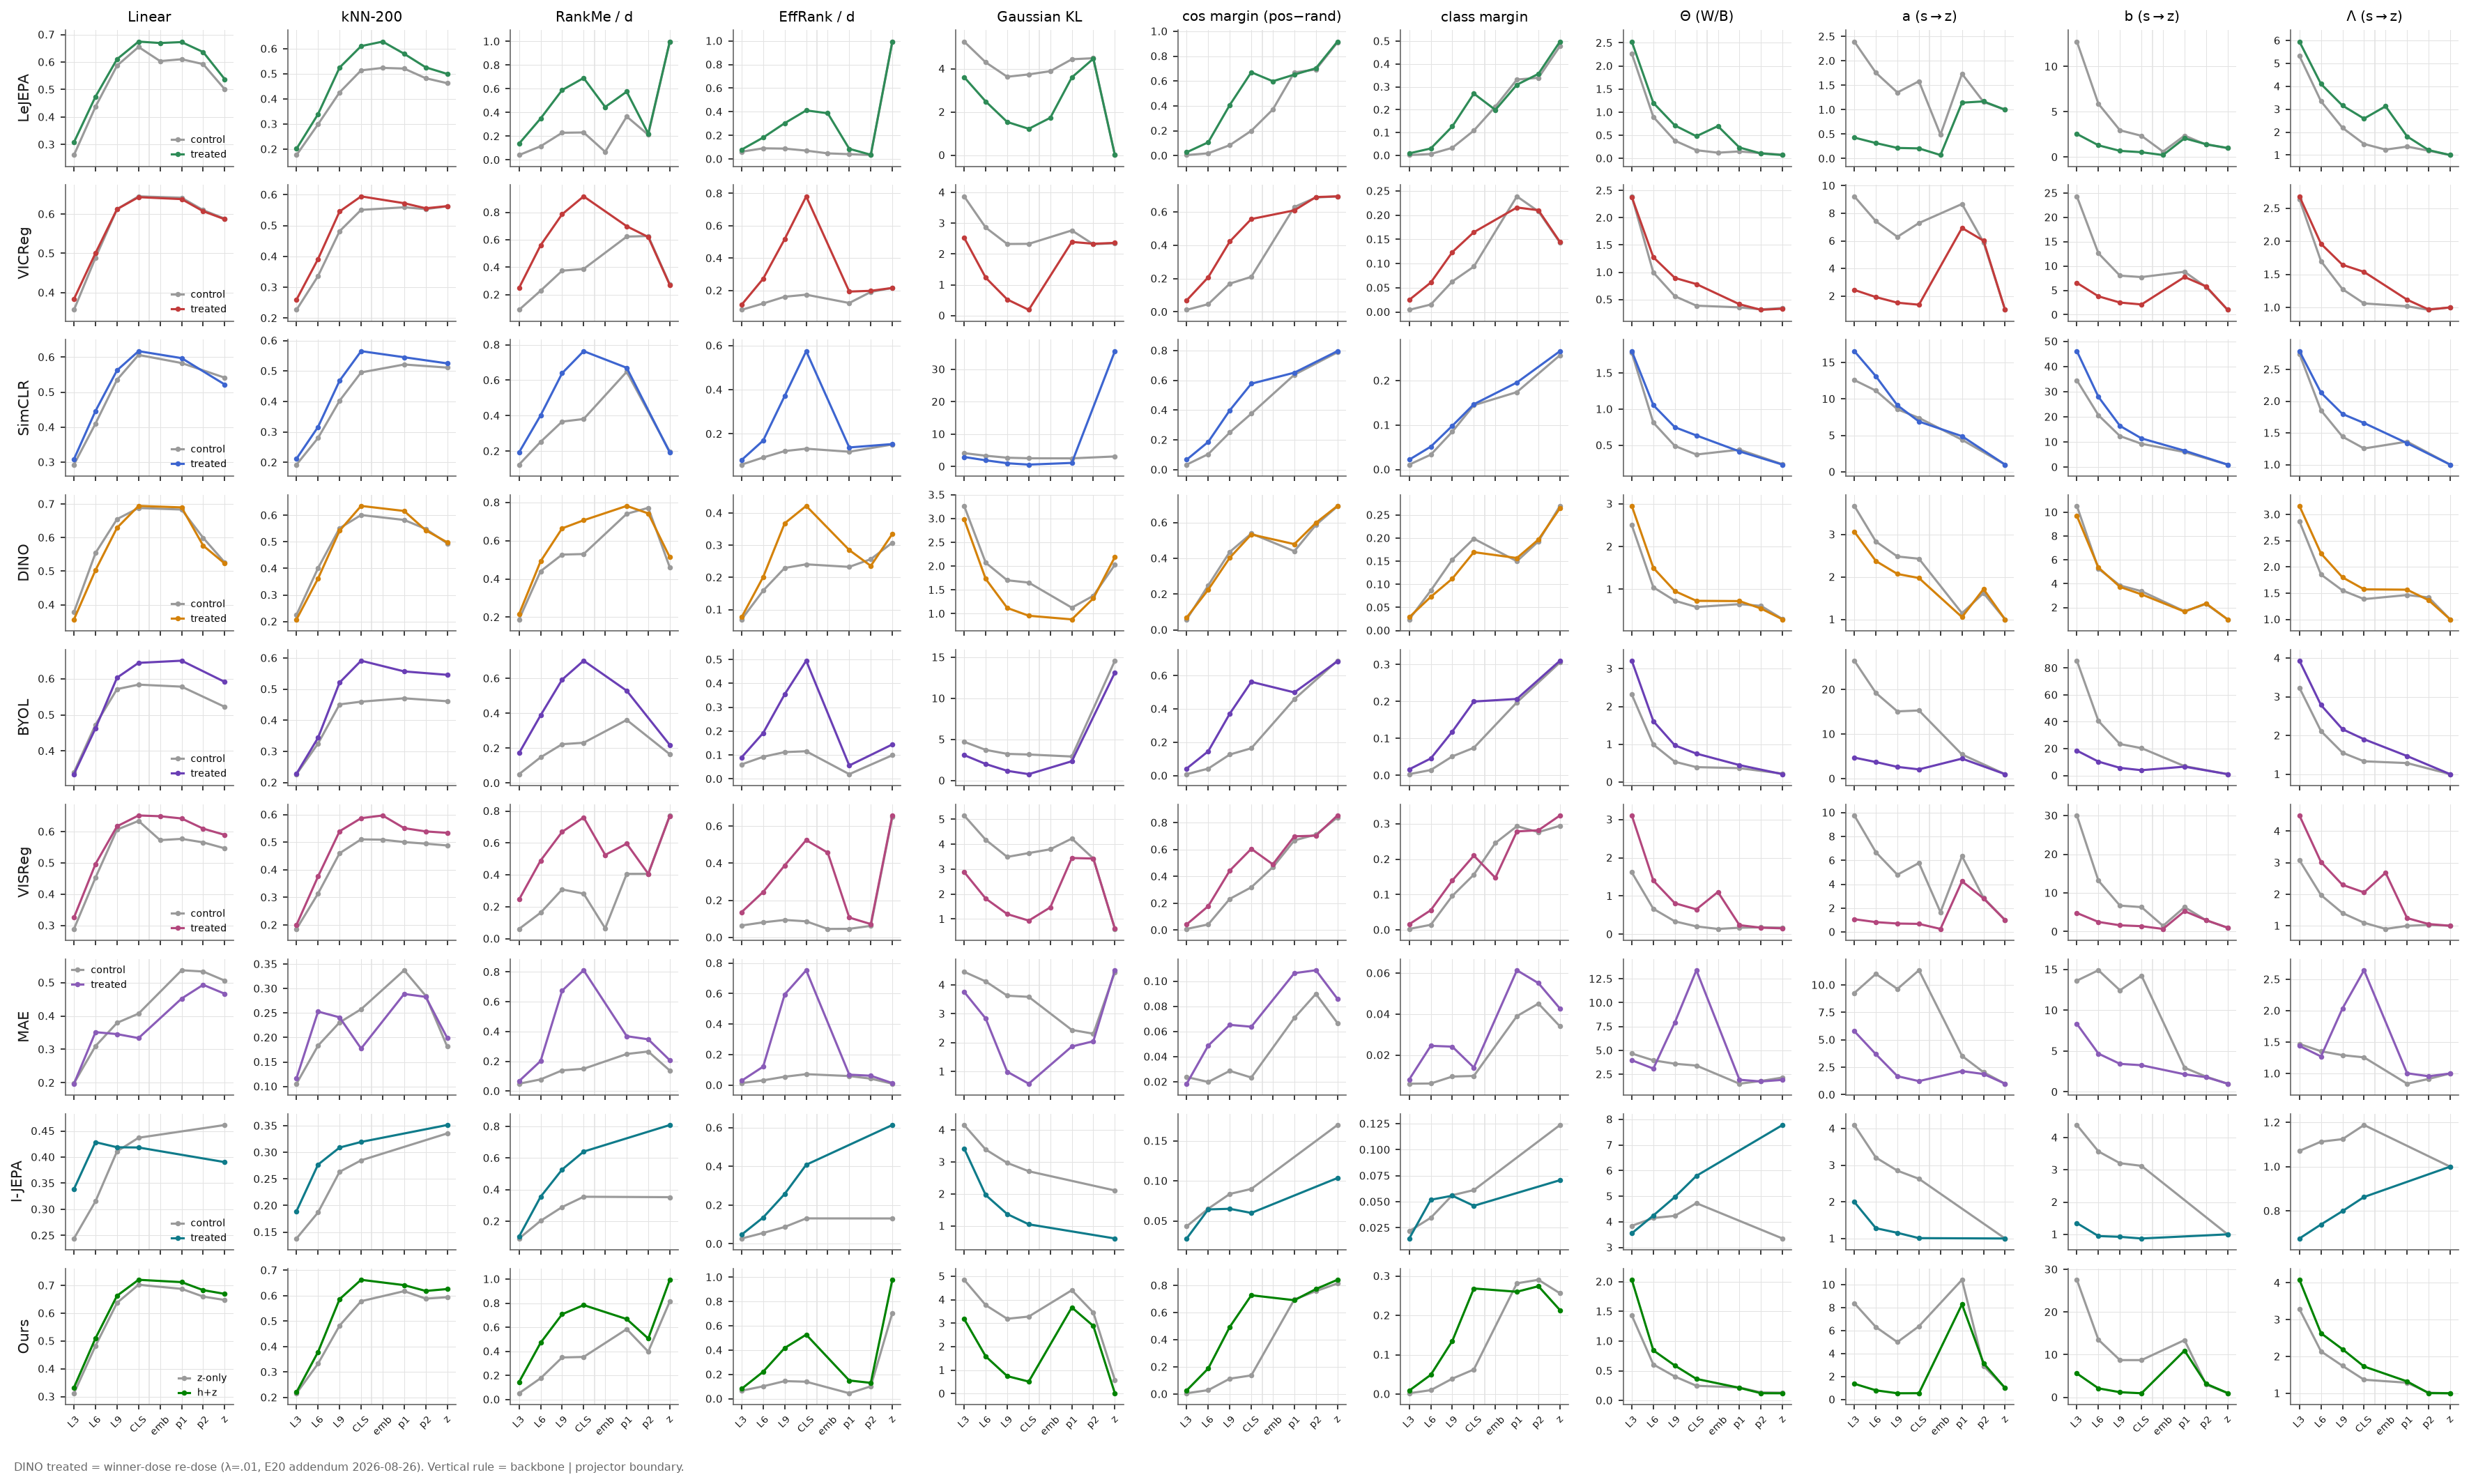
\includegraphics[width=\linewidth]{figures/fig_treatment_appendix.png}
  \caption{}\label{fig:treatment-appendix}
\end{figure}


\section{The fidelity law: certifying the meter}\label{app:fidelity-law}
% SKELETON (C4, ruled appendix 2026-08-25): held-out residual spectrum of the train-fit
% single-view->center map vs Theta(I+Theta)^{-1} + Theta/V, per direction in Theta's
% eigenbasis; log-corr .993+ over three decades, all four methods, both spaces; the
% +1-16% small-lambda deviations = the finite-sample estimation floor (n ~ 10k), stated;
% linearity-of-conditional-mean caveat + the planted-nonlinearity MLP control, presented
% as a caveat, not a claim.

\section{Structured and residual view-sensitivity}\label{app:gs-split}
% SKELETON (C5, de-emphasized per 2026-08-25 ruling): the G/S decomposition measured,
% never graded; neutral language only ("beyond what representing the centers requires").

\section{Accessibility over training}\label{app:trajectories}
% SKELETON (C6): within-run trajectories (dimension constant over time); cross-method
% levels only after the per-run dimension-matched null correction (R^2 minus shuffled-
% target null). Claim wording ruled: standard SSL slowly erodes the h->z bridge over
% training; ours improves it.
